\section{NUMERICAL EXPERIMENTS}
\label{sec:numerics}

\subsection{Models and Evaluation Protocol}

The phase-map QRCs have two, three, or four qubits, random $XX$ couplings,
transverse fields, input-dependent drives, and local loss $\gamma_T$.
Inputs use a uniform 33-point alphabet on $[0,1]$; outputs are single-site
Pauli expectations and same-axis two-site correlations.  A fixed six-qubit
reset-QELM encodes $d\leq6$ recent inputs, evolves under independent random
$XX$ couplings, and records Pauli features at nested times.  We vary $d$,
feature budget $B\in\{18,36,72\}$, and circuit shots per input $Q$.
This fixed emulator is not the theorem's growing universal family.
The Appendix specifies the dynamics and training parameters.

An independent realization block, or root, fixes the target, streams, and
feature map.  Training, validation, test, and diagnostic streams are
separate.  Training determines standardization; validation selects the ridge
readout.  The confirmatory two- and three-qubit cohort has 12 roots.
The denser loss--window map uses disjoint seeds; a prospectively frozen
four-qubit follow-up has 12 new roots.  Cohorts are never pooled.

A held-out common-suffix panel combines different old histories with
identical recent inputs.  Their mean squared output variation is the
old-history term; the squared distance from their mean to the window
prediction is the residual emulator error.  These add exactly to panel
MSE [Eq.~\eqref{eq:panel-decomposition}].  This distribution-dependent
diagnostic does not estimate worst-case $D_d$ or $r_{\rm vis}$ directly.

\begin{figure*}[t]
 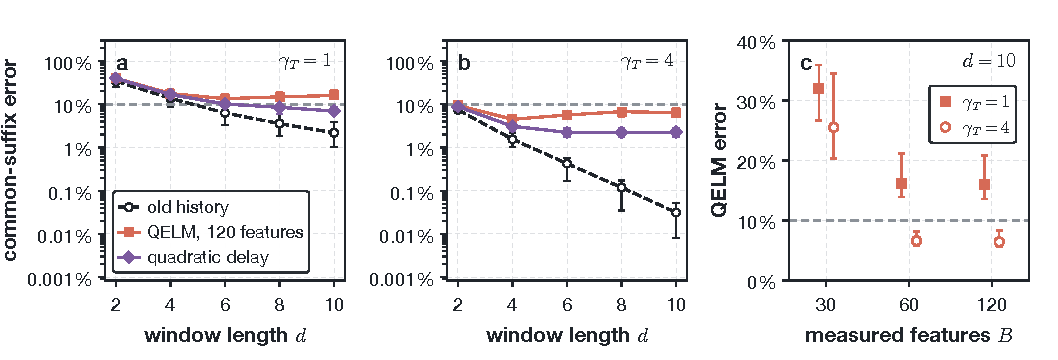
\includegraphics[width=\textwidth]{fig04_long_context_n5.pdf}
 \caption{Five-qubit targets and longer context.
 Separate prospective cohort: 12 new roots, a fixed ten-qubit reset-QELM,
 and all tested windows at $\gamma_T=1$ (a) and 4 (b).
 Common-suffix NRMSE compares the history floor, fixed $B=120$ QELM,
 and quadratic delay. Lines show root medians; whiskers span the
 10th--90th percentiles. The key applies to both panels; the gray dashed line marks 10\%.
 The larger register is an additional resource, not a matched-size advantage.}
 \label{fig:long-context}
\end{figure*}

Normalized RMSE (NRMSE) $0.10$ means 10\% of the target standard deviation.
A frontier cell succeeds when at least 10 of 12 roots meet this tolerance.
Confidence intervals use paired root-block bootstraps, not individual rows
or repeated measurements.

\subsection{History, Representation, and Measurement Limits}

The three questions are whether the window contains enough history, whether
features represent its output map, and whether shots resolve those features.
Under weak loss, old prefixes influence the output throughout the tested
window range.  Increasing loss shifts the measured frontier toward shorter
windows.  Across preregistered transition cells ($B=72$,
$\gamma_T\in\{2,4\}$), increasing $d=1\to6$ reduces held-out QELM NRMSE by a root median of $78.45\%$ (95\% CI
$[76.64,80.80]\%$), with the same direction in all 12 roots.

The dense maps test 11 loss rates and all integer windows from one to six:
198 cells across the two- and three-qubit cohort and the separately frozen
four-qubit follow-up.
Every rootwise local-loss decay fit has negative slope in both confirmatory
sizes.  The independent four-qubit cohort also has negative slopes and a
non-increasing frontier; every root reaches the inherited
$\gamma_T=4,d=6,B=72$ anchor.  Across all three sizes, no tested window is
history-sufficient through $\gamma_T=1$; the minimum falls to two by
$\gamma_T=4$.  The tested minimum history windows coincide across sizes, while
minimum successful feature budgets and emulation outcomes differ.
For each size at $\gamma_T=2,B=72$, $d=5$ meets the total-error root rule
but $d=6$ does not.
This is a tested loss--window crossover, not an asymptotic size law.

The primary $0.10$, 10-of-12 rule was preregistered.  A post hoc check uses
tolerances $0.08$, $0.10$, and $0.12$ with 9, 10, or 11 required roots.
Crossing cells change, but all 27 measured, right-censored
size--tolerance--rule frontiers remain non-increasing with loss.

On the fast-forgetting slice, limits appear in sequence.  At
$d=1,B=72$, all roots are history limited.  At $d=6,B=18$, the history
target is met but the fixed QELM is usually representation limited in the
operational sense defined in Section~\ref{sec:methods}. At
$d=6,B=36$, every root across all three sizes reaches the tolerance.
Figure~\ref{fig:resource-diagnosis}(b) shows the feature dependence for the
two- and three-qubit targets.

On the history-sufficient slice $\gamma_T=4,d=6$, increasing the QELM budget
from $B=18$ to 72 reduces common-suffix residual emulator NRMSE by a root median
of $67.26\%$ (95\% CI $[55.33,75.63]\%$), with the same direction in all 12
roots and both confirmatory sizes.  At $B=72$, all 24 confirmatory
root-by-size cases are emulated.  Features do not change the old-history term.

The exploratory post-confirmatory shot study independently samples training,
validation, and test features; target outputs remain exact expectations.
Validation-selected test NRMSE falls from
$0.231$ at 300 shots per input to $0.0800$ at 19,200 shots, a $65.20\%$
reduction (95\% CI $[64.04,66.47]\%$), positive in all 12 roots.  Validation
selects $B=36$ most often at low shot counts and $B=72$ at high shot counts.
Extra features help when the measurement budget resolves them
[Figure~\ref{fig:resource-diagnosis}(c)]
\cite{hu2023sampling,ahmed2025finite}.

Linear delay, quadratic delay, and dimension-matched random-tanh controls use
the same windows and splits as the QELM.  Quadratic delay is the strongest
classical control in all 24 fast-forgetting confirmatory cases and outperforms
the $B=72$ QELM in every root. This is a resource diagnosis,
not quantum advantage.

With five-qubit targets and a ten-qubit reset-QELM
(Figure~\ref{fig:long-context}), increasing $d=2\to10$ reduces history NRMSE
by root medians of $93.55\%$ at $\gamma_T=1$ and $99.63\%$ at
$\gamma_T=4$, positive in all 12 roots at each loss.
At $\gamma_T=1$, windows 6, 8, and 10 meet the history rule but no tested
QELM budget meets the total-error rule. At $\gamma_T=4$, every window meets
the history rule; $B=60$ reaches the total-error target in all 12 roots
only from $d=4$ onward. Quadratic delay beats the fixed $B=120$ QELM in
118 of 120 streaming root--condition comparisons.
